% -----------------------------------------------------------------------------------------
% -----------------------------------------------------------------------------------------
% Current file is a modified version of the original TeX file,
% which was written by Paul Torfs & Claudia Brauer.
% It's the basic file for the greek translation of their respective
% introductory tutorial in R, "A (very) short introduction to R".
% -----------------------------------------------------------------------------------------
% -----------------------------------------------------------------------------------------

\documentclass[a4paper,11pt,twocolumn,tablecaptionabove]{scrartcl}

\usepackage{amssymb}
\bibliographystyle{plain}
\usepackage{multicol}
\usepackage{rotating}
\usepackage{url}
\usepackage{hyperref}
\usepackage{multirow}
\usepackage{a4wide}
\usepackage{graphicx}
\usepackage{wasysym}

% packages for R-intro chapter
\usepackage{pkg/fancybox}
\usepackage{pkg/fvrb-ex}

\usepackage[top=2.4cm, bottom=2.4cm, left=2cm, right=2cm]{geometry}
\setkomafont{captionlabel}{\bfseries} %% Bold float caption
\setcapindent{1em}

% -----------------------------------------------------------------------------------------
% Additions for greek language. -----------------------------------------------------------
\usepackage{fontspec}
\usepackage{xunicode}
\usepackage{xltxtra}
\usepackage{xgreek}
\setmainfont[Mapping=TeX-text]{Times New Roman}
% -----------------------------------------------------------------------------------------

% format of footnotes
\renewcommand{\thefootnote}{\fnsymbol{footnote}} % sets the footnotesymbols to fn in stead of numbers (already in use)
\deffootnote[1em]{0em}{1em}{\textsuperscript{\thefootnotemark}}

%%
%% The ToDo environment
%%
\usepackage[usenames,dvipsnames]{color}
 \newenvironment{ToDo} {%
  \begin{flushright}
    \hfill
    \begin{minipage}{0.95\columnwidth}         % used to be 0.95\columnwidth
    \textsf{\textbf{ToDo}} \\
      \vspace{-0.85cm}\\
      {\color{Gray}\rule[-0.1cm]{\columnwidth}{1.5pt}}} { % used to  be without 0.1cm
      {\color{Gray} \rule[0.3cm]{\columnwidth}{1.5pt}}
    \end{minipage}
    \vspace{1em}
  \end{flushright}
  }  
%%  

\makeatletter

\newcommand{\noun}[1]{\textsc{#1}}
%% Special footnote code from the package 'stblftnt.sty'
%% Author: Robin Fairbairns -- Last revised Dec 13 1996
\let\SF@@footnote\footnote
\def\footnote{\ifx\protect\@typeset@protect
 \expandafter\SF@@footnote
 \else
 \expandafter\SF@gobble@opt
 \fi
}
\expandafter\def\csname SF@gobble@opt \endcsname{\@ifnextchar[%]
 \SF@gobble@twobracket
 \@gobble
}
\edef\SF@gobble@opt{\noexpand\protect
 \expandafter\noexpand\csname SF@gobble@opt \endcsname}
\def\SF@gobble@twobracket[#1]#2{}

%%%%%%%%%%%%%%%%%%%%%%%%%%%%%%

\makeatother

% improve float handling
\renewcommand{\topfraction}{0.9}	
 \renewcommand{\bottomfraction}{0.8}	
 \setcounter{topnumber}{2}
 \setcounter{bottomnumber}{2}
 \setcounter{totalnumber}{4} 
 \setcounter{dbltopnumber}{2} 
 \renewcommand{\dbltopfraction}{0.9}	
 \renewcommand{\textfraction}{0.07}	
 \renewcommand{\floatpagefraction}{0.7}	
	% floatpagefraction MUST be less than topfraction !!
 \renewcommand{\dblfloatpagefraction}{0.7}

% change : to . in float caption
\renewcommand*{\captionformat}{\ } 

% package for making question boxes
\usepackage{boxedminipage}

% -----------------------------------------------------------------------------------------
% NOTES ON FORMATTING
% \texttt{...} is used to emphasize commands or clicking buttons in verbatim.
% \verb!...! is only used instead of \texttt{...} when there are brackets or other things
% \texttt can't handle.
% \emph is used to emphasize new terms
% -----------------------------------------------------------------------------------------

\title{\vspace{-13mm}A (very) short introduction to R}
\author{Paul Torfs \& Claudia Brauer\\
\footnotesize{Ομάδα Υδρολογίας και Ποσοτικής Διαχείρισης Υδάτων}\\
\footnotesize{Πανεπιστήμιο Wageningen, Ολλανδία}}
\date{\small{4 Νοεμβρίου 2014}}

\begin{document}

\maketitle

% -----------------------------------------------------------------------------------------
% [#01] 
% -----------------------------------------------------------------------------------------
\section{Introduction}

Η R είναι μια ισχυρή γλώσσα και ένα ισχυρό περιβάλλον ανάπτυξης για στατιστικούς
υπολογισμούς και γραφικά. Ως έργο είναι κοινό κτήμα (ή αλλιώς είναι ένα λεγόμενο ``GNU" project),
το οποίο είναι παρόμοιο με την εμπορική γλώσσα και περιβάλλον S, που είχε αναπτυχθεί στα Bell 
Laboratories (πρώην AT\&T, πλέον Lucent Technologies) από τον John Chambers και τους συνεργάτες
του. Η R μπορεί να θεωρηθεί πως είναι μια διαφορετική υλοποίηση της S, και χρησιμοποιείται ευρέως
ως εκπαιδευτική γλώσσα και ερευνητικό εργαλείο.

Τα κύρια πλεονεκτήματα της R είναι το γεγονός ότι η R αποτελεί ελεύθερο λογισμικό και ότι υπάρχει
πολύ βοήθεια διαθέσιμη στο διαδίκτυο. Είναι αρκετά παρόμοια με άλλα προγραμματιστικά πακέτα όπως 
η MATLAB (που δεν είναι ελεύθερο λογισμικό), αλλά πιο φιλική προς τον χρήστη από γλώσσες
προγραμματισμού όπως η C++ και η Fortran. Μπορείτε να χρησιμοποιήσετε την R όπως είναι, αλλά για
εκπαιδευτικούς λόγους εμείς προτιμούμε τη χρήση της R σε συνδυασμό με την διεπαφή του RStudio (που είναι επίσης ελεύθερο λογισμικό), το οποίο έχει μια οργανωμένη διάταξη και διάφορες πρόσθετες
επιλογές.

Το παρόν έγγραφο περιλαμβάνει επεξηγήσεις, παραδείγματα και ασκήσεις, τα οποία (ελπίζουμε ότι)
μπορούν να γίνουν κατανοητά από ανθρώπους χωρίς καμία προγραμματιστική εμπειρία. Το διάβασμα
όλου του κειμένου και των ασκήσεων απαιτεί περίπου 1 με 2 ώρες. Παραδείγματα από εντολές που 
χρησιμοποιούνται συχνά και από μηνύματα λάθους παρατίθενται στις τελευταίες δύο σελίδες αυτού
του εγγράφου και μπορούν να χρησιμοποιηθούν ως αναφορά κατά τον προγραμματισμό.

% ------------------------------------------------------------------------------------------------------------------------------------
% [#02] ----------------------------------------------------------------------------------------------------------------------------
\section{Getting started}

%%% [.01] -----------------------------------------------------------------------------------
\subsection{Install R}

Για να εγκαταστήσετε την R στον υπολογιστή σας (δωρεάν και με νόμιμο τρόπο!), πηγαίνετε στην
αρχική σελίδα του ιστοτόπου της R\footnote{Στον ιστότοπο της R μπορείτε επίσης να βρείτε και αυτό το παρόν έγγραφο: \url{http://cran.r-project.org/doc/contrib/Torfs+Brauer-Short-R-Intro.pdf}}:
\begin{quote}
  \url{http://www.r-project.org/}
\end{quote}
και εκτελέστε τα ακόλουθα (υποθέτοντας ότι δουλεύετε σε έναν υπολογιστή με Windows):\\
\noindent $\bullet$ κάντε κλικ στο \texttt{download CRAN} στην αριστερή στήλη\\
\noindent $\bullet$ επιλέξτε έναν ιστότοπο  για το download\\
\noindent $\bullet$ επιλέξτε \texttt{Windows} ως λειτουργικό σύστημα\\
\noindent $\bullet$ κάντε κλικ στο \texttt{base}\\
\noindent $\bullet$ επιλέξτε \texttt{Download R 3.0.3 for Windows} \footnote{Τη στιγμή της
συγγραφής του κειμένου αυτού η τελευταία έκδοση ήταν η 3.0.3. Επιλέξτε την πιο πρόσφατη.} και
αφήστε τις προεπιλεγμένες απαντήσεις σε όλες τις ερωτήσεις\\

Είναι επίσης πιθανό να εκτελέσετε την R και το RStudio από ένα USB αντί να τα εγκαταστήσετε. Αυτό
θα μπορούσε να είναι χρήσιμο όταν δεν έχετε δικαιώματα διαχειριστή στον υπολογιστή σας. Δείτε και 
την ξεχωριστή σημείωσή μας ``How to use portable versions of R and RStudio" για βοήθεια στο 
συγκεκριμένο θέμα.

%%% [.02] -----------------------------------------------------------------------------------
\subsection{Install RStudio}

Μετά την ολοκλήρωση της εγκατάστασης, θα πρέπει να βλέπετε ένα εικονίδιο "R" στην επιφάνεια
εργασίας σας. Κάνοντας κλικ σε αυτό θα εκκινήσετε την τυπική διεπαφή. Εμείς θα συνιστούσαμε,
ωστόσο, να χρησιμοποιήσετε την διεπαφή του RStudio. \footnote{Υπάρχουν πολλές άλλες διεπαφές
(ελεύθερου λογισμικού), όπως το Tinn-R.} Για να εγκαταστήσετε το RStudio, πηγαίνετε στον ιστότοπο: 
\begin{quote}
  \url{http://www.rstudio.org/}
\end{quote}
και εκτελέστε τα ακόλουθα (υποθέτοντας ότι δουλεύετε σε έναν υπολογιστή με Windows):\\
\noindent $\bullet$ κάντε κλικ στο \texttt{Download RStudio}\\
\noindent $\bullet$ κάντε κλικ στο \texttt{Download RStudio Desktop}\\
\noindent $\bullet$ κάντε κλικ στο \texttt{Recommended For Your System}\\
\noindent $\bullet$ κατεβάστε το \texttt{.exe} αρχείο και τρέξτε το 
(αφήστε τις προεπιλεγμένες απαντήσεις για όλες τις ερωτήσεις)

%%% [.03] -----------------------------------------------------------------------------------
\subsection{RStudio layout}

\begin{figure*}[htb]
  \centering
  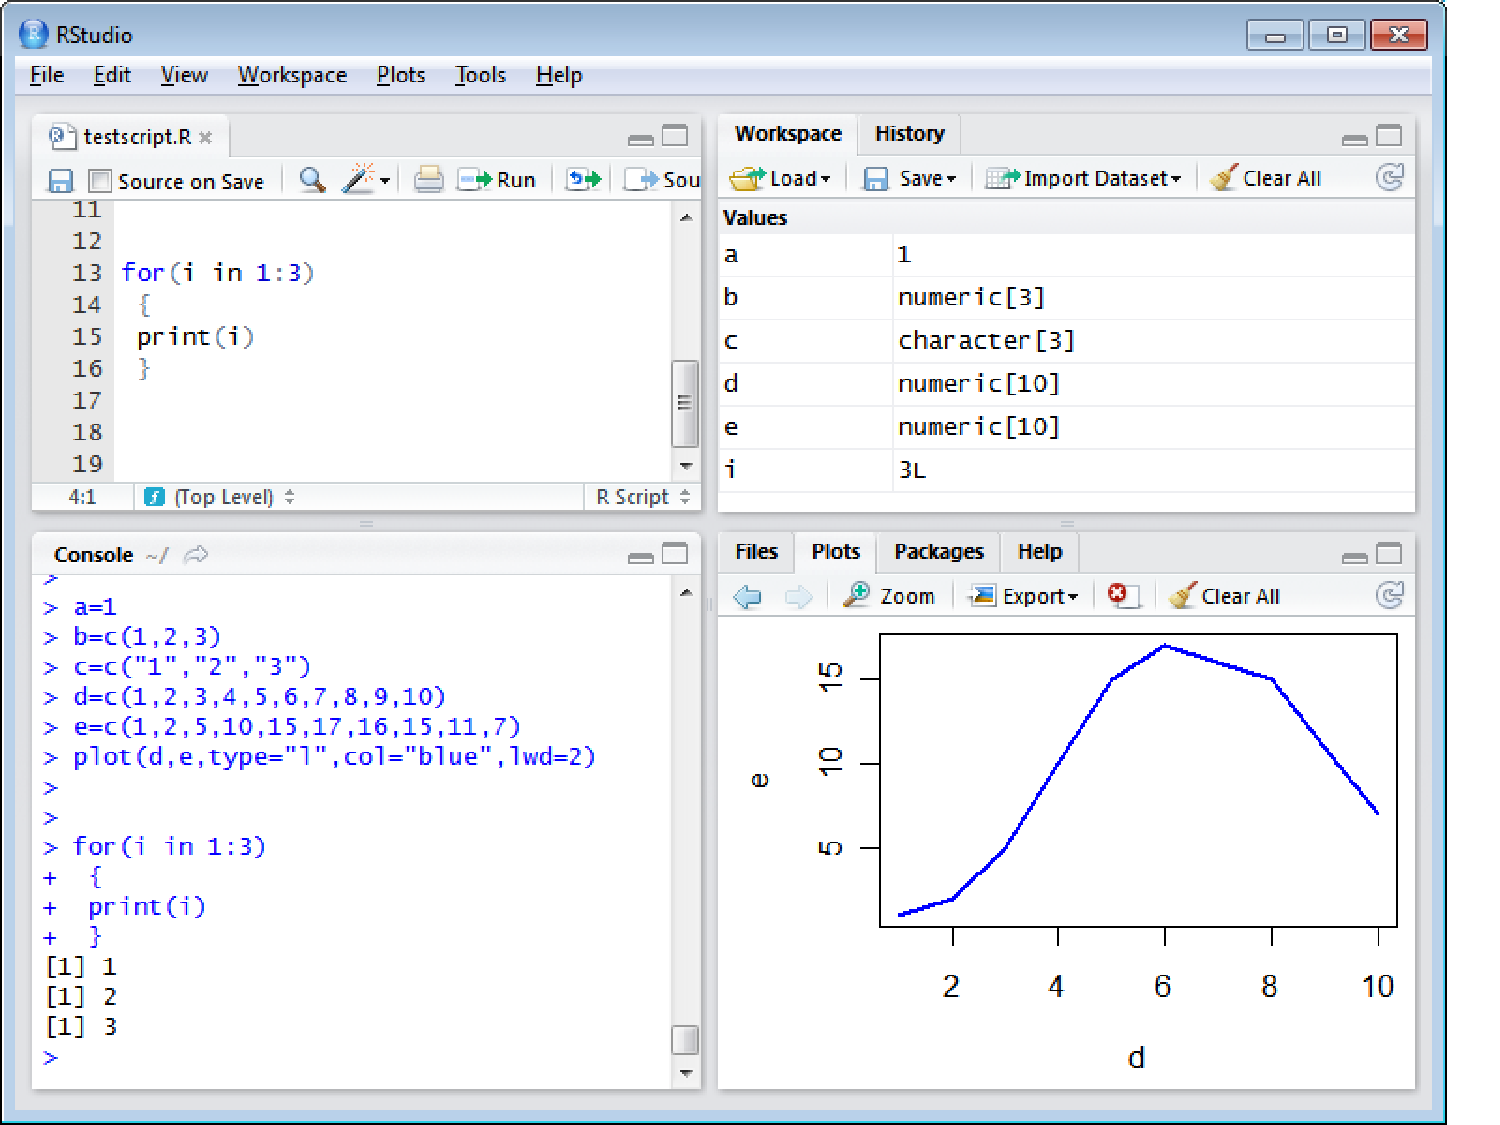
\includegraphics[width=13cm, clip=true, trim=0cm 0cm 9mm 0cm]{img/rstudio_screenshot.pdf}
  \caption{Τα παράθυρα του επεργαστή κειμένου, του χώρου εργασίας, της κονσόλας και των γραφικών παραστάσεων στο RStudio.}
  \label{fig:screenshot}
\end{figure*}

Η διεπαφή του RStudio αποτελείται από διάφορα παράδειγμα (βλέπε το Σχήμα~\ref{fig:screenshot}).
\begin{itemize}
\item Κάτω αριστερά: \textbf{παράθυρο κονσόλας} (που καλείται επίσης και \textbf{παράθυρο εντολών}). H
Εδώ μπορείτε να εισάγετε απλές εντολές μετά το σύμβολο υποβολής ``$>$'' και η R στη συνέχεια θα εκτελέσει
εντολή σας. Αυτό είναι το πιο σημαντικό παράθυρο, επειδή στην πραγματικότητα εκεί τρέχει η R.
\item Πάνω αριστερά: \textbf{παράθυρο επεξεργαστή κειμένου} (που καλείται επίσης και \textbf{παράθυρο σεναρίων}).
Εδώ μπορούν να υποστούν επεξεργασία και να σωθούν σύνολα από εντολές (σενάρια). Όταν δεν υπάρχει αυτό το
παράθυρο, μπορείτε να το ανοίξετε μέσω \texttt{File} $\rightarrow$ \texttt{New} $\rightarrow$ \texttt{R script}\\
Η απλή πληκτρολόγηση μιας εντολής στο παράθυρο του επεξεργαστή δεν είναι αρκετή, πρέπει επίσης να πάει και στο
παράθυρο εντολών πριν η R μπορέσει να εκτελέσει την εντολή αυτή. Εάν θέλετε να τρέξετε μία γραμμή από το 
παράθυρο σεναρίων (ή και ολόκληρο το σενάριο), μπορείτε να κάνετε κλικ στο \texttt{Run} ή να πατήσετε τα
πλήκτρα \texttt{CTRL+ENTER} ώστε να τη στείλετε στο παράθυρο εντολών. 
\item Πάνω δεξιά: \textbf{χώρος εργασίας / ιστορικό}. Στο παράθυρο του χώρου εργασίας
μπορείτε να δείτε ποια δεδομένα και ποιες τιμές έχει η R στη μνήμη της. Μπορείτε να δείτε και να επεξεργαστείτε
τις τιμές κάνοντας κλικ πάνω τους. Το παράθυρο του ιστορικού δείχνει το τι έχει πληκτρολογηθεί παλιότερα. 
\item Κάτω δεξιά: \textbf{αρχεία / γραφικές παραστάσεις / πακέτα / βοήθεια}. Από εδώ μπορείτε να ανοίξετε
αρχεία, να δείτε γραφικές παραστάσεις (και προηγούμενες γραφικές παραστάσεις, επίσης), να εγκαταστήσετε
και να φορτώσετε πακέτα ή να χρησιμοποιήσετε τη λειτουργία της βοήθειας.
\end{itemize}

Μπορείτε να αλλάξετε το μέγεθος των παραθύρων σέρνοντας τα γκρίζα διαχωριστικά μεταξύ των παραθύρων.

%%% [.04] -----------------------------------------------------------------------------------
\subsection{Working directory}

Ο \emph{κατάλογος εργασίας} σας είναι ο φάκελος του υπολογιστή σας μέσα στον οποίο εργάζεστε. Όταν ζητάτε από
την R να ανοίξει ένα συγκεκριμένο αρχείο, αυτή θα κοιτάξει πρώτα στον κατάλογο εργασίας γι' αυτό το αρχείο, και
όταν πείτε στην R να αποθηκεύσει ένα αρχείο δεδομένων ή ένα γράφημα, αυτή θα το αποθηκεύσει στον κατάλογο
εργασίας.

Πριν ξεκινήσετε να εργάζεστε, παρακαλούμε θέστε τον κατάλογο εργασίας σας εκεί που έχετε ή εκεί που πρέπει
να αποθηκεύονται όλα τα δεδομένα σας και τα αρχεία σεναρίων.

Εισάγετε στο παράθυρο εντολών το εξής: \verb!setwd("directoryname")!. Για παράδειγμα:
\begin{Verbatim}[frame=single,gobble=0]
> setwd("M:/Hydrology/R/")
\end{Verbatim}
Σιγουρευτείτε ότι οι μπάρες είναι πλάγιες μπάρες (/) και ότι δεν έχετε ξεχάσει τις αποστρόφους (για την ανάγκη
των αποστρόφων, δείτε στην ενότητα~\ref{sec:characters}). Η R διακρίνει τα πεζά από τα κεφαλαία γράμματα, οπότε
βεβαιωθείτε ότι γράφετε με κεφαλαία εκεί που απαιτείται.

Μέσα στο RStudio μπορείτε επίσης να πάτε στο \texttt{Tools / Set working directory}.

%%% [.05] -----------------------------------------------------------------------------------
\subsection{Libraries} 

Η R μπορεί να κάνει πολλές στατιστικές αναλύσεις και αναλύσεις δεδομένων. Αυτές είναι οργανωμένες στα 
λεγόμενα \emph{πακέτα} ή \emph{βιβλιοθήκες}. Με την τυπική εγκατάσταση, εγκαθίστανται και τα περισσότερα
συνήθη πακέτα. 

Για να δείτε μια λίστα με όλα τα εγκατεστημένα πακέτα, πηγαίνετε στο παράθυρο πακέτων ή πληκτρολογήστε 
\verb!library()! στο παράθυρο κονσόλας. Εάν το τετραγωνάκι μπροστά από το όνομα του πακέτου είναι τικαρισμένο,
το πακέτο φορτώνεται (ενεργοποιείται) και τότε μπορεί να χρησιμοποιηθεί. 

Υπάρχουν πολλά επιπλέον πακέτα διαθέσιμα στον ιστότοπο της R. Εάν θέλετε να εγκαταστήσετε και να χρησιμοποιήσετε
ένα πακέτο (για παράδειγμα, το πακέτο που λέγεται ``geometry"), τότε πρέπι να :\\
\noindent $\bullet$ Εγκαταστήσετε το πακέτο:  κάντε κλικ στο \texttt{install packages} στο παράθυρο πακέτων
και πληκτρολογήστε \texttt{geometry} ή εισάγετε την εντολή \verb!install.packages("geometry")! στο παράθυρο
εντολών.\\
\noindent $\bullet$ Φορτώστε το πακέτο: επιλέξτε το κουτάκι μπροστά από το \texttt{geometry} ή εισάγετε
την εντολή \verb!library("geometry")! στο παράθυρο εντολών.


% ------------------------------------------------------------------------------------------------------------------------------------
% [#03] ----------------------------------------------------------------------------------------------------------------------------
\section{Some first examples of R commands}

%%% [.01] -----------------------------------------------------------------------------------
\subsection{Calculator}

R can be used as a calculator. You can just type your equation in the command window after the ``$>$":
\begin{Verbatim}[frame=single,gobble=0]
> 10^2 + 36
\end{Verbatim}
and R will give the answer
\begin{Verbatim}[frame=single,gobble=0]
[1] 136
\end{Verbatim}

\begin{ToDo}
Compute the difference between 2014 and the year you started at this university and divide this by the difference between 2014 and the year you were born. Multiply this with 100 to get the percentage of your life you have spent at this university. Use brackets if you need them. \\
\end{ToDo}

If you use brackets and forget to add the closing bracket, the ``$>$" on the command line changes into a ``+". The ``+" can also mean that R is still busy with some  heavy computation. If you want R to quit what it was doing and give back the ``$>$", press \texttt{ESC} (see the reference list on the last page). 

%%% [.02] -----------------------------------------------------------------------------------
\subsection{Workspace}

You can also give numbers a name. By doing so, they become so-called variables which can be used later. For example, you can type in the command window: 
\begin{Verbatim}[frame=single,gobble=0]
> a = 4
\end{Verbatim}
You can see that \texttt{a} appears in the workspace window, which means that R now remembers what \texttt{a} is.\footnote{Some people prefer te use \texttt{<-} instead of \texttt{=} (they do the same thing). \texttt{<-} consists of two characters, \texttt{<} and \texttt{-}, and represents an arrow pointing at the object receiving the value of the expression.} You can also ask R what \texttt{a} is (just type \texttt{a ENTER} in the command window):

\begin{Verbatim}[frame=single,gobble=0]
> a 
[1] 4
\end{Verbatim}
or do calculations with \texttt{a}: 

\begin{Verbatim}[frame=single,gobble=0]
> a * 5
[1] 20
\end{Verbatim}

If you specify \texttt{a} again, it will forget what value it had before. You can also assign a new value to \texttt{a} using the old one.

\begin{Verbatim}[frame=single,gobble=0]
> a = a + 10
> a
[1] 14
\end{Verbatim}

To remove all variables from R's memory, type
\begin{Verbatim}[frame=single,gobble=0]
> rm(list=ls())
\end{Verbatim}
or click ``clear all" in the workspace window. You can see that RStudio then empties the workspace window. If you only want to remove the variable \texttt{a}, you can type \texttt{rm(a)}.

\begin{ToDo}
Repeat the previous ToDo, but with several steps in between. You can give the variables any name you want, but the name has to start with a letter. \\
\end{ToDo}

%%% [.03] -----------------------------------------------------------------------------------
\subsection{Scalars, vectors and matrices}

Like in many other programs, R organizes numbers in \emph{scalars} (a single number -- 0-dimensional), \emph{vectors} (a row of numbers, also called arrays -- 1-dimensional) and \emph{matrices} (like a table -- 2-dimensional).

The \texttt{a} you defined before was a scalar. To define a vector with the numbers 3, 4 and 5, you need the function\footnote{See next Section for the explanation of functions.} \texttt{c}, which is short for concatenate (paste together). 
\begin{Verbatim}[frame=single,gobble=0]
b=c(3,4,5)
\end{Verbatim}

Matrices and other 2-dimensional structures will be introduced in Section~\ref{sec:structures}.

%%% [.04] -----------------------------------------------------------------------------------
\subsection{Functions}

If you would like to compute the mean of all the elements in the vector \texttt{b} from the example above, you could type 
\begin{Verbatim}[frame=single,gobble=0]
> (3+4+5)/3
\end{Verbatim}
But when the vector is very long, this is very boring and time-consuming work. This is why things you do often are automated in so-called \emph{functions}. Some functions are standard in R or in one of the packages. You can also program your own functions (Section~\ref{sec:progfunc}). When you use a function to compute a mean, you'll type:
\begin{Verbatim}[frame=single,gobble=0]
> mean(x=b)
\end{Verbatim}

Within the brackets you specify the \emph{arguments}. Arguments give extra information to the function. In this case, the argument \texttt{x} says of which set of numbers (vector) the mean should computed (namely of \texttt{b}). Sometimes, the name of the argument is not necessary: \texttt{mean(b)} works as well.

\begin{ToDo}
Compute the sum of 4, 5, 8 and 11 by first combining them into a vector and then using the function \texttt{sum}.\\
\end{ToDo}

\begin{figure*}[htb]
  \centering
  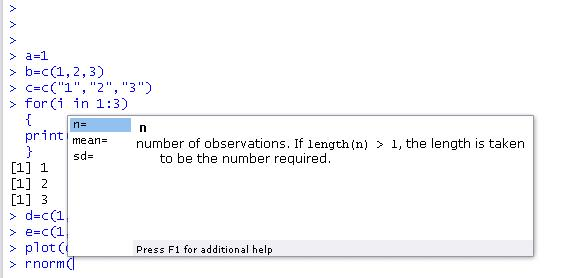
\includegraphics[width=10cm, clip=true, trim=0cm 0cm 0cm 1cm]{img/tab_RStudio.jpg}
  \caption{RStudio shows possible arguments when you press \texttt{TAB} after the function name and bracket.}
  \label{fig:tab_RStudio}
\end{figure*}

The function \texttt{rnorm}, as another example, is a standard R function which creates random samples from a normal distribution.  Hit the \texttt{ENTER} key and you will see 10 random numbers as:

\begin{Verbatim}[frame=single,numbers=left,gobble=0, xleftmargin=0.35cm, numbersep=0.1cm]
> rnorm(10)
[1] -0.949  1.342 -0.474 0.403 
[5] -0.091 -0.379  1.015  0.740 
[9] -0.639  0.950
\end{Verbatim}

\noindent $\bullet$ Line 1 contains the command: \texttt{rnorm} is the function and the 10 is an argument specifying how many random numbers you want --- in this case 10 numbers (typing \texttt{n=10} instead of just \texttt{10} would also work).\\
\noindent $\bullet$  Lines 2-4 contain the results: 10 random numbers organised in a vector with length 10.

Entering the same command again produces 10 new random numbers. Instead of typing the same text again, you can also press the upward arrow key ($\uparrow$) to access previous commands.  If you want 10 random numbers out of normal distribution with mean 1.2 and standard deviation 3.4 you can type 
\begin{Verbatim}[frame=single,gobble=0]
> rnorm(10, mean=1.2, sd=3.4)
\end{Verbatim}
showing that the same function (\texttt{rnorm}) may have different interfaces and that R has so called \emph{named arguments}  (in this case \texttt{mean} and \texttt{sd}). By the way, the spaces around the ``," and ``=" do not matter.

Comparing this example to the previous one also shows that for the function \texttt{rnorm} only the first argument (the number 10) is compulsory, and that R gives default values to the other so-called optional arguments.\footnote{Use the help function (Sect.~\ref{sec:help}) to see which values are used as default.} 

RStudio has a nice feature: when you type \verb!rnorm(! in the command window and press \texttt{TAB}, RStudio will show the possible arguments (Fig.~\ref{fig:tab_RStudio}).

%%% [.05] -----------------------------------------------------------------------------------
\subsection{Plots}

R can make graphs. The following is a very simple~\footnote{See Section~\ref{sec:some-plotting} for slightly less trivial examples.}
example:
\begin{Verbatim}[frame=single,numbers=left,gobble=0, xleftmargin=0.35cm, numbersep=0.1cm]
> x = rnorm(100)
> plot(x)
\end{Verbatim}

\noindent $\bullet$ In the first line, 100 random numbers are assigned to the variable \texttt{x}, which becomes a vector by this operation. \\
\noindent $\bullet$ In the second line, all these
values are  plotted in the plots window.\\

\begin{ToDo}
Plot 100 normal random numbers.\\
\end{ToDo}


% ------------------------------------------------------------------------------------------------------------------------------------
% [#04] ----------------------------------------------------------------------------------------------------------------------------
\section{Help and documentation}
\label{sec:help}

There is a large amount of (free) documentation and help available. 
Some help is automatically installed. Typing in the console window the command
\begin{Verbatim}[frame=single,gobble=0]
> help(rnorm)
\end{Verbatim}
gives help on the \texttt{rnorm} function. It gives a description of the function, possible arguments and the values that are used as default for optional arguments. Typing
\begin{Verbatim}[frame=single,gobble=0]
> example(rnorm)
\end{Verbatim}
gives some examples of how the function can be used. 

An HTML-based global help can be called with:
\begin{Verbatim}[frame=single,gobble=0]
> help.start()
\end{Verbatim}
or by going to the help window.

The following links can also be very useful:\\
\noindent $\bullet$ \url{http://cran.r-project.org/doc/manuals/ R-intro.pdf} A full manual.\\
\noindent $\bullet$ \url{http://cran.r-project.org/doc/contrib/ Short-refcard.pdf} A short reference card.\\
\noindent $\bullet$  \url{http://zoonek2.free.fr/UNIX/48\_R/all.html}\\
  A very rich source of examples.\\
\noindent $\bullet$  \url{http://rwiki.sciviews.org/doku.php}\\
  A typical user wiki.\\
\noindent $\bullet$ \url{http://www.statmethods.net/}\\
    Also called Quick-R. Gives very productive direct help. Also for users coming from other programming languages. \\
    \noindent $\bullet$ \url{http://mathesaurus.sourceforge.net/}\\
    Dictionary for programming languages (e.g.~R for Matlab users). \\
\noindent $\bullet$  Just using Google (type e.g. ``R rnorm'' in the search field) can also be very
productive.\\

\begin{ToDo}
Find help for the \texttt{sqrt} function.\\
\end{ToDo}


% ------------------------------------------------------------------------------------------------------------------------------------
% [#05] ----------------------------------------------------------------------------------------------------------------------------
\section{Scripts}

R is an interpreter that uses a command line based environment. This means that you have to type
commands, rather than use the mouse and menus.  
This has the advantage that you do not always have to retype all commands and are less likely to get complaints of arms, neck and shoulders.

You can store your commands in files, the so-called \emph{scripts}.  
These scripts have typically file names with the extension
\texttt{.R}, e.g.  \texttt{foo.R}.  
You can open an editor window to edit these
files by clicking \texttt{File} and \texttt{New} or \texttt{Open file...}
\footnote{Where also the options \texttt{Save} and
  \texttt{Save as} are available.}.

You can run (send to the console window) part of the code by selecting lines and pressing \texttt{CTRL+ENTER} or click \texttt{Run} in the editor window.
If you do not select anything, R will run the line your cursor is on.
You can always  run the whole script with the console command \texttt{source},
so e.g. for the script in the file \texttt{foo.R} you type:
\begin{Verbatim}[frame=single,gobble=0]
> source("foo.R")
\end{Verbatim}
You can also click \texttt{Run all} in the editor window or type \texttt{CTRL+SHIFT + S} to run the whole script at once.

\begin{ToDo}
  Make a file called \texttt{firstscript.R} containing R-code that generates 100
  random numbers and plots them, and run this script several times.\\
\end{ToDo}


% ------------------------------------------------------------------------------------------------------------------------------------
% [#06] ----------------------------------------------------------------------------------------------------------------------------
\section{Data structures} 
\label{sec:structures}

If you are unfamiliar with R, it makes sense to just retype the commands
listed in this section. Maybe you will not need all these structures in the
beginning, but it is always good to have at least a first glimpse of the
terminology and possible applications.

%%% [.01] -----------------------------------------------------------------------------------
\subsection{Vectors}

\emph{Vectors} were already introduced, but they can do more:

\begin{Verbatim}[frame=single,numbers=left,gobble=0, xleftmargin=0.35cm, numbersep=0.1cm]
> vec1 = c(1,4,6,8,10)
> vec1
[1]  1  4  6  8 10
> vec1[5]
[1] 10
> vec1[3] = 12
> vec1
[1]  1  4 12  8 10
> vec2 = seq(from=0, to=1, by=0.25)
> vec2
[1] 0.00 0.25 0.50 0.75 1.00
> sum(vec1)
[1] 35
> vec1 + vec2
[1]  1.00 4.25 12.50 8.75 11.00
\end{Verbatim}

\noindent $\bullet$  In line 1, a vector \texttt{vec1} is explicitly constructed by the concatenation function \texttt{c()}, which was introduced before. Elements in vectors can be addressed by standard \texttt{[i]} indexing, as shown in lines 4-5. \\
\noindent $\bullet$  In line 6, one of the elements is replaced with a new number. The result is shown in line 8.\\
\noindent $\bullet$ Line 9 demonstrates another useful way of constructing a vector: the \texttt{seq()} (sequence) function. \\
\noindent $\bullet$ Lines 10-15 show some typical vector oriented calculations. If you add up two vectors of the same length, the first elements of both vectors are summed, and the second elements, etc., leading to a new vector of length 5 (just like in regular vector calculus). Note that the function \texttt{sum} sums up the elements within a vector, leading to one number (a scalar).

%%% [.02] -----------------------------------------------------------------------------------
\subsection{Matrices}

\emph{Matrices} are nothing more than 2-dimensional vectors. To define a matrix, use the function \texttt{matrix}:
\begin{Verbatim}[frame=single,numbers=left,gobble=0, xleftmargin=0.35cm, numbersep=0.1cm]
mat=matrix(data=c(9,2,3,4,5,6),ncol=3)
> mat
     [,1] [,2] [,3]
[1,]    9    3    5
[2,]    2    4    6
\end{Verbatim}

The argument \texttt{data} specifies which numbers should be in the matrix. Use either  \texttt{ncol} to specify the number of columns or \texttt{nrow} to specify the number of rows. 

\begin{ToDo}
Put the numbers 31 to 60 in a vector named \texttt{P} and in a matrix with 6 rows and 5 columns named \texttt{Q}. Tip: use the function \texttt{seq}. Look at the different ways scalars, vectors and matrices are denoted in the workspace window.\\
\end{ToDo}
 
 Matrix-operations are similar to vector operations:

\begin{Verbatim}[frame=single,numbers=left,gobble=0, xleftmargin=0.35cm, numbersep=0.1cm]
> mat[1,2]
[1] 3
> mat[2,]
[1] 2 4 6
> mean(mat)
[1] 4.8333
\end{Verbatim}

\noindent $\bullet$ Elements of a matrix can be addressed in the usual way: \texttt{[row,column]} (line 1). \\
\noindent $\bullet$ Line 3: When you want to select a whole row, you leave the spot for the column number empty (the other way around for columns of course).\\
\noindent $\bullet$ Line 5 shows that many functions also work with matrices as argument.\\

%%% [.03] -----------------------------------------------------------------------------------
\subsection{Data frames}

Time series are often ordered in \emph{data frames}. A data frame is a matrix with names above the columns. This is nice, because you can call and use one of the columns without knowing in which position it is.
\begin{Verbatim}[frame=single,numbers=left,gobble=0, xleftmargin=0.35cm, numbersep=0.1cm]
> t = data.frame(x = c(11,12,14),
 y = c(19,20,21), z = c(10,9,7))
> t
   x y z
1 11 19 10
2 12 20 9 
3 14 21 7  
> mean(t$z)
[1] 8.666667
> mean(t[["z"]])
[1] 8.666667
\end{Verbatim}
%%$

\noindent $\bullet$ In lines 1-2 a typical data frame called \texttt{t} is constructed. The columns have the names \texttt{x}, \texttt{y} and \texttt{z}.\\
\noindent $\bullet$ Line 8-11 show two ways of how you can select the column called \texttt{z} from the data frame called \texttt{t}.\\
\\

\begin{ToDo}
Make a script file which constructs three random normal vectors of length 100. Call these vectors \texttt{x1}, \texttt{x2} and \texttt{x3}. Make a data frame called \texttt{t} with three columns (called \texttt{a}, \texttt{b} and \texttt{c}) containing respectively \texttt{x1}, \texttt{x1+x2} and \texttt{x1+x2+x3}. Call the following functions for this data frame: \texttt{plot(t)} and \texttt{sd(t\$x1)}. Can you understand the results? Rerun this script a few times.\\
\end{ToDo}

%%% [.04] -----------------------------------------------------------------------------------
\subsection{Lists}

Another basic structure in R is a \emph{list}. The main advantage of lists is that the ``columns" (they're not really ordered in columns any more, but are more a collection of vectors) don't have to be of the same length, unlike matrices and data frames. 

\begin{Verbatim}[frame=single,numbers=left,gobble=0, xleftmargin=0.35cm, numbersep=0.1cm]
> L = list(one=1, two=c(1,2), 
 five=seq(0, 1, length=5))
> L
$one
[1] 1
$two
[1] 1 2
$five
[1] 0.00 0.25 0.50 0.75 1.00
> names(L)
[1] "one"  "two"  "five"
> L$five + 10
[1] 10.00 10.25 10.50 10.75 11.00
\end{Verbatim}

\noindent $\bullet$ Lines 1-2 construct a list by giving names and values. The list also appears in the workspace window.\\
\noindent $\bullet$ Lines 3-9 show a typical printing (after pressing \texttt{L ENTER}). \\
\noindent $\bullet$ Line 10 illustrates how to find out what's in the list.\\
\noindent $\bullet$ Line 12 shows how to use the numbers. \\


% ------------------------------------------------------------------------------------------------------------------------------------
% [#07] ----------------------------------------------------------------------------------------------------------------------------
\section{Graphics}
\label{sec:some-plotting}

Plotting is an important statistical activity. So it should not come as a
surprise that R has many plotting facilities. 
The following lines show a simple plot:
\begin{Verbatim}[frame=single,gobble=0]
> plot(rnorm(100), type="l", col="gold")
\end{Verbatim}

\noindent Hundred random numbers are plotted by connecting the points by lines (the
symbol between quotes after the \texttt{type=}, is the letter l, not the
number 1) in a gold color.

Another very simple example is the classical statistical histogram plot, generated by the
simple command
\begin{Verbatim}[frame=single,gobble=0]
  > hist(rnorm(100))
\end{Verbatim}
which generates the plot in Figure~\ref{fig:hist}.
\begin{figure}[h]
  \centering
  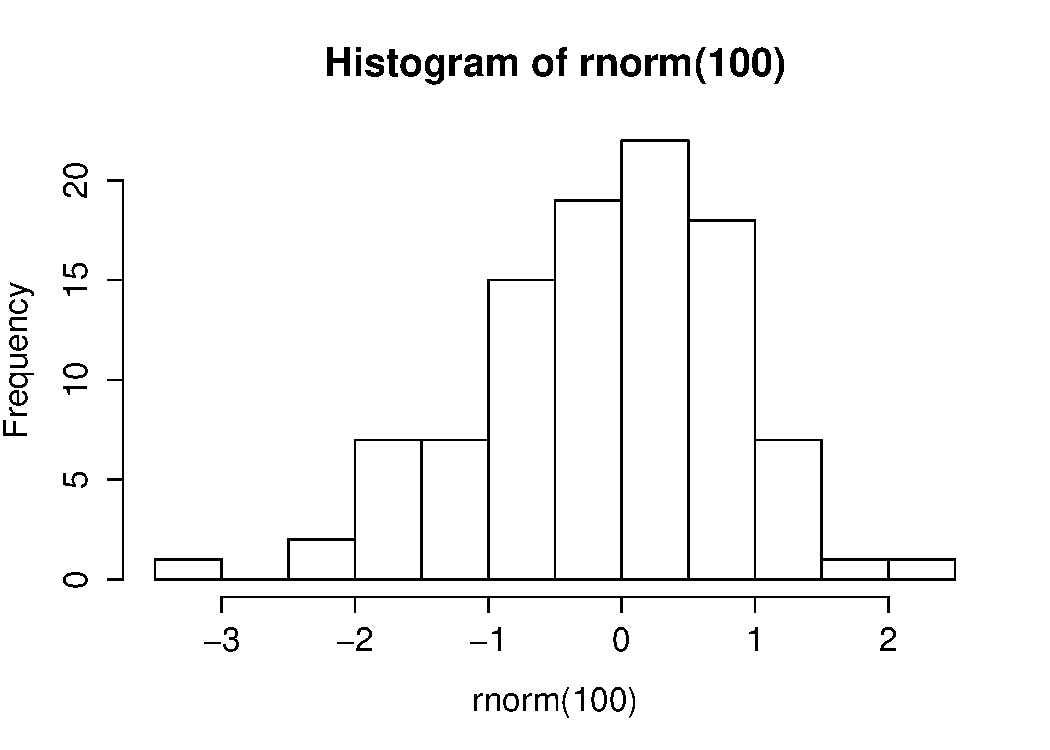
\includegraphics[width=8cm]{img/hist.pdf}
  \caption{A simple histogram plot.}
  \label{fig:hist}
\end{figure}

\noindent The following few lines create a plot using the data frame \texttt{t}
constructed in the previous ToDo:
\begin{Verbatim}[frame=single,numbers=left,gobble=0, xleftmargin=0.35cm, numbersep=0.1cm]
plot(t$a, type="l", ylim=range(t), 
 lwd=3, col=rgb(1,0,0,0.3))
lines(t$b, type="s", lwd=2, 
 col=rgb(0.3,0.4,0.3,0.9))
points(t$c, pch=20, cex=4, 
 col=rgb(0,0,1,0.3))
\end{Verbatim} 
%%$ 

\begin{ToDo}
  Add these lines to the script file of the previous section. Try to
  find out, either by experimenting or by using the help, what the
  meaning is of \texttt{rgb}, the last argument of \texttt{rgb},
  \texttt{lwd}, \texttt{pch}, \texttt{cex}.\\
\end{ToDo}

To learn more about formatting plots, search for \texttt{par} in the R help. 
Google ``R color chart" for a pdf file with a wealth of color options.

To copy your plot to a document, go to the plots window, click the ``Export" button, choose the nicest width and height and click \texttt{Copy} or \texttt{Save}. 


% ------------------------------------------------------------------------------------------------------------------------------------
% [#08] ----------------------------------------------------------------------------------------------------------------------------
\section{Reading and writing data files}
\label{sec:reading-writing-data}

There are many ways to write data from within the R environment to files, and to read data from files. We will illustrate one way here. The following lines illustrate the essential:

\begin{Verbatim}[frame=single,numbers=left,gobble=0, xleftmargin=0.35cm, numbersep=0.1cm]
> d = data.frame(a = c(3,4,5), 
 b = c(12,43,54))
> d
  a  b
1 3 12
2 4 43
3 5 54
> write.table(d, file="tst0.txt",
 row.names=FALSE)
> d2 = read.table(file="tst0.txt", 
 header=TRUE)
> d2
  a  b
1 3 12
2 4 43
3 5 54
\end{Verbatim}
\noindent $\bullet$ In lines 1-2, a simple example data frame is constructed and stored in the
variable \texttt{d}. \\
\noindent $\bullet$ Lines 3-7 show the content of this data frame: two columns (called \texttt{a} and \texttt{b}), each containing three numbers.\\
\noindent $\bullet$ Line 8 writes this data frame to a text file, called \texttt{tst0.txt} The argument
\verb!row.names=FALSE! prevents that row names are written to the file. Because nothing is specified about \texttt{col.names}, the default option \verb!col.names=TRUE! is chosen
and column names are written to the file. Figure~\ref{fig:tst0}
shows the resulting file (opened in an editor, such as Notepad), with the
column names (\texttt{a} and \texttt{b}) in the first line. \\
\noindent $\bullet$ Lines 10-11 illustrate how to read a file into a data frame. Note that the column names are also read. The data frame also appears in the workspace window.\\

\begin{figure}[h]
  \centering
  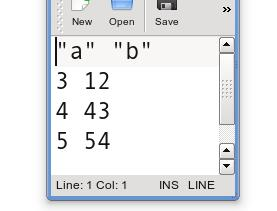
\includegraphics[width=3.5cm]{img/tst0.jpeg}
  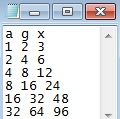
\includegraphics[width=2.6cm]{img/tst1.jpg}
  \caption{The files \texttt{tst0.txt} of section~\ref{sec:reading-writing-data}
    (left) and \texttt{tst1.txt} from the ToDo below (right) opened in two text editors.}
  \label{fig:tst0}
\end{figure}

\begin{ToDo}
  Make a file called \texttt{tst1.txt} in Notepad from the example in Figure~\ref{fig:tst0} and store it in your working directory. Write a
  script to read it, to multiply the column called \texttt{g} by 5 and to store it as
  \texttt{tst2.txt}.\\
\end{ToDo}


% ------------------------------------------------------------------------------------------------------------------------------------
% [#09] ----------------------------------------------------------------------------------------------------------------------------
\section{Not available data}

\begin{ToDo}
Compute the mean of the square root of a vector of 100 random numbers. What happens? 
\end{ToDo}

When you work with real data, you will encounter missing values because instrumentation failed or because you didn't want to measure in the weekend. When a data point is \emph{not available}, you write \texttt{NA} instead of a number. 

\begin{Verbatim}[frame=single,gobble=0]
> j = c(1,2,NA)
\end{Verbatim}

Computing statistics of incomplete data sets is strictly speaking not possible. Maybe the largest value occurred during the weekend when you didn't measure. Therefore, R will say that it doesn't know what the largest value of \texttt{j} is: 

\begin{Verbatim}[frame=single,gobble=0]
> max(j)
[1] NA
\end{Verbatim}

If you don't mind about the missing data and want to compute the statistics anyway, you can add the argument \texttt{na.rm=TRUE} (Should I remove the NAs? Yes!). 

\begin{Verbatim}[frame=single,gobble=0]
> max(j, na.rm=TRUE)
[1] 2
\end{Verbatim}


% ------------------------------------------------------------------------------------------------------------------------------------
% [#10] ----------------------------------------------------------------------------------------------------------------------------
\section{Classes}

The exercises you did before were nearly all with numbers. Sometimes you want to specify something which is not a number, for example the name of a measurement station or data file. In that case you want the variable to be a character string instead of a number. 

An object in R can have several so-called \emph{classes}. The most important three are
\emph{numeric}, \emph{character} and \emph{POSIX} (date-time combinations). You can ask R what class a certain variable is by typing \texttt{class(...)}. 

%%% [.01] -----------------------------------------------------------------------------------
\subsection{Characters}
\label{sec:characters}

To tell R that something is a character string, you should type the text between apostrophes, otherwise R will start looking for a defined variable with the same name:

\begin{Verbatim}[frame=single,gobble=0]
> m = "apples"
> m
[1] "apples"
> n = pears
Error: object `pears' not found
\end{Verbatim}

Of course, you cannot do computations with character strings:

\begin{Verbatim}[frame=single,gobble=0]
> m + 2
Error in m + 2 : non-numeric argument to 
binary operator
\end{Verbatim}

%%% [.02] -----------------------------------------------------------------------------------
\subsection{Dates}

Dates and times are complicated. R has to know that 3 o'clock comes after 2:59 and that February has 29~days in some years. The easiest way to tell R that something is a date-time combination is with the function \texttt{strptime}:

\begin{Verbatim}[frame=single,numbers=left,gobble=0, xleftmargin=0.35cm, numbersep=0.1cm]
> date1=strptime( c("20100225230000", 
 "20100226000000", "20100226010000"), 
 format="%Y%m%d%H%M%S")
 > date1
[1] "2010-02-25 23:00:00" 
[2] "2010-02-26 00:00:00" 
[3] "2010-02-26 01:00:00"
\end{Verbatim}

\noindent $\bullet$  In lines 1-2 you create a vector with \texttt{c(...)}. The numbers in the vectors are between apostrophes because the function \texttt{strptime} needs character strings as input.\\
\noindent $\bullet$ In line 3 the argument \texttt{format} specifies how the character string should be read. In this case the year is denoted first (\%Y), then the month (\%m), day (\%d), hour (\%H), minute (\%M) and second (\%S). You don't have to specify all of them, as long as the format corresponds to the character string.

\begin{ToDo}
Make a graph with on the x-axis: today, Sinterklaas 2014 and your next birthday and on the y-axis the number of presents you expect on each of these days. Tip: make two vectors first.
\end{ToDo}

%You can also plot dates (for example on the x-axis), as shown by the following code, which yields %Figure~\ref{fig:date}:

%\begin{Verbatim}[frame=single,gobble=0]
%> y=c(1,6,8)
%> plot(date1,y)
%\end{Verbatim}

%\begin{figure}[h]
%  \centering
%  \includegraphics[width=\columnwidth]{date_plot}
%  \caption{Plotting dates on the x-axis.}
%  \label{fig:date}
%\end{figure}


% ------------------------------------------------------------------------------------------------------------------------------------
% [#11] ----------------------------------------------------------------------------------------------------------------------------
\section{Programming tools}

When you are building a larger program than in the examples above or if you're using someone else's scripts, you may encounter some programming statements. In this Section we describe a few tips and tricks.

%%% [.01] -----------------------------------------------------------------------------------
\subsection{If-statement}

The \emph{if-statement} is used when certain computations should \emph{only} be done when a certain condition is met (and maybe something else should be done when the condition is not met). An example:

\begin{Verbatim}[frame=single,numbers=left,gobble=0, xleftmargin=0.35cm, numbersep=0.1cm]
> w = 3
> if( w < 5 )
   {
   d=2
   }else{
   d=10
   }
> d
2
\end{Verbatim}

\noindent $\bullet$ In line 2 a condition is specified: \texttt{w} should be less than 5.\\
\noindent $\bullet$ If the condition is met, R will execute what is between the first brackets in line 4.\\
\noindent $\bullet$ If the condition is \emph{not} met, R will execute what is between the second brackets, after the \texttt{else} in line 6. You can leave the \verb!else{...}!-part out if you don't need it.\\
\noindent $\bullet$ In this case, the condition is met and \texttt{d} has been assigned the value 2 (lines 8-9).

To get a subset of points in a vector for which a certain condition holds, you can use a shorter method:

\begin{Verbatim}[frame=single,numbers=left,gobble=0, xleftmargin=0.35cm, numbersep=0.1cm]
> a = c(1,2,3,4)
> b = c(5,6,7,8)
> f = a[b==5 | b==8]
> f
[1] 1 4
\end{Verbatim}

\noindent $\bullet$ In line 1 and 2 two vectors are made.\\
\noindent $\bullet$ In line 3 you say that \texttt{f} is composed of those elements of vector \texttt{a} for which \texttt{b} equals 5 or \texttt{b} equals 8. \\

Note the double \texttt{=} in the condition. Other conditions (also called logical or Boolean operators) are \texttt{<}, \texttt{>}, \texttt{!=} ($\neq$), \texttt{<=} ($\leq$) and \texttt{>=} ($\geq$). To test more than one condition in one if-statement, use \texttt{\&} if both conditions have to be met (``and") and \texttt{|} if one of the conditions has to be met (``or").

%%% [.02] -----------------------------------------------------------------------------------
\subsection{For-loop}

If you want to model a time series, you usually do the computations for one time step and then for the next and the next, etc. Because nobody wants to type the same commands over and over again, these computations are automated in for-loops. 

In a \emph{for-loop} you specify what has to be done and how many times. To tell ``how many times", you specify a so-called counter. An example:

\begin{Verbatim}[frame=single,numbers=left,gobble=0, xleftmargin=0.35cm, numbersep=0.1cm]
> h = seq(from=1, to=8)
> s = c()
> for(i in 2:10) 
   {
   s[i] = h[i] * 10
   }
> s
[1] NA 20 30 40 50 60 70 80 NA NA
\end{Verbatim}

\noindent $\bullet$ First the vector  \texttt{h} is made.\\
\noindent $\bullet$ In line 2 an empty vector ( \texttt{s}) is created. This is necessary because when you introduce a variable within the for-loop, R will not remember it when it has gotten out of the for-loop.\\
\noindent $\bullet$  In line 3 the for-loop starts. In this case, \texttt{i} is the counter and runs from 2 to 10.\\
\noindent $\bullet$ Everything between the curly brackets (line 5) is processed 9 times. The first time \texttt{i=2}, the second element of \texttt{h} is multiplied with 10 and placed in the second position of the vector \texttt{s}. The second time \texttt{i=3}, etc. In the last two runs, the 9$^\mathrm{th}$ and 10$^\mathrm{th}$ elements of \texttt{h} are requested, which do not exist. Note that these statements are evaluated without any explicit error messages.

\begin{ToDo}
Make a vector from 1 to 100. Make a for-loop which runs through the whole vector. Multiply the elements which are smaller than 5 and larger than 90 with 10 and the other elements with 0.1.
\end{ToDo}

%%% [.03] -----------------------------------------------------------------------------------
\subsection{Writing your own functions}
\label{sec:progfunc}

Functions you program yourself work in the same way as pre-programmed R functions.

\begin{Verbatim}[frame=single,numbers=left,gobble=0, xleftmargin=0.35cm, numbersep=0.1cm]
> fun1 = function(arg1, arg2 )
   {
   w = arg1 ^ 2
   return(arg2 + w)
   }
> fun1(arg1 = 3, arg2 = 5) 
[1] 14

\end{Verbatim}

\noindent $\bullet$ In line 1 the function name (\texttt{fun1}) and its arguments (\texttt{arg1} and \texttt{arg2}) are defined. \\
\noindent $\bullet$ Lines 2-5 specify what the function should do if it is called. The return value (\texttt{arg2+w}) is shown on the screen. \\
\noindent $\bullet$ In line 6 the function is called with arguments 3 and 5.

\begin{ToDo}
Write a function for the previous ToDo, so that you can feed it any vector you like (as argument). Use a for-loop in the function to do the computation with each element. Use the standard R function \texttt{length} in the specification of the counter. \footnote{Actually, people often use more for-loops than necessary. The ToDo above can be done more easily and quickly without a for-loop but with regular vector-computations.})
\end{ToDo}

\newpage


% ------------------------------------------------------------------------------------------------------------------------------------
% [#12] ----------------------------------------------------------------------------------------------------------------------------
\section{Some useful references}

%%% [.01] -----------------------------------------------------------------------------------
\subsection{Functions}

This is a subset of the functions explained in the R reference card.\\

\noindent \underline{Data creation}\\
$\bullet$ \texttt{read.table}: read a table from file. Arguments: \texttt{header=TRUE}: read first line as titles of the columns; \texttt{sep=","}: numbers are separated by commas; \texttt{skip=n}: don't read the first \texttt{n} lines.\\
$\bullet$ \texttt{write.table}: write a table to file\\
$\bullet$ \texttt{c}: paste numbers together to create a vector\\
$\bullet$ \texttt{array}: create a vector, Arguments: \texttt{dim}: length
$\bullet$ \texttt{matrix}: create a matrix, Arguments: \texttt{ncol} and/or \texttt{nrow}: number of rows/columns\\
$\bullet$ \texttt{data.frame}: create a data frame\\
$\bullet$ \texttt{list}: create a list\\
$\bullet$ \texttt{rbind} and \texttt{cbind}: combine vectors into a matrix by row or column\\

\noindent \underline{Extracting data}\\
$\bullet$ \texttt{x[n]}: the \texttt{n}$\mathrm{^{th}}$ element of a vector\\
$\bullet$ \texttt{x[m:n]}: the \texttt{m}$\mathrm{^{th}}$ to \texttt{n}$\mathrm{^{th}}$ element\\
$\bullet$ \texttt{x[c(k,m,n)]}: specific elements\\
$\bullet$ \texttt{x[x>m \& x<n]}: elements between \texttt{m} and \texttt{n}\\
$\bullet$ \verb!x$n!:  element of list or data frame named \texttt{n}\\  %$
$\bullet$ \texttt{x[["n"]]}: idem\\
$\bullet$ \texttt{[i,j]}: element at \texttt{i}$\mathrm{^{th}}$ row and\texttt{ }j$\mathrm{^{th}}$ column \\
$\bullet$ \texttt{[i,]}: row \texttt{i} in a matrix\\

\noindent \underline{Information on variables}\\
$\bullet$ \texttt{length}: length of a vector\\
$\bullet$ \texttt{ncol} or \texttt{nrow}: number of columns or rows in a matrix\\
$\bullet$ \texttt{class}: class of a variable \\
$\bullet$ \texttt{names}: names of objects in a list \\
$\bullet$ \texttt{print}: show variable or character string on the screen (used in scripts or for-loops) \\
$\bullet$ \texttt{return}: show variable on the screen (used in functions) \\
$\bullet$ \texttt{is.na}: test if variable is \texttt{NA}\\
$\bullet$ \texttt{as.numeric} or \texttt{as.character}: change class to number or character string\\
$\bullet$ \texttt{strptime}: change class from character to date-time (POSIX)\\

\noindent \underline{Statistics}\\
$\bullet$ \texttt{sum}: sum of a vector (or matrix)\\
$\bullet$ \texttt{mean}: mean of a vector\\
$\bullet$ \texttt{sd}: standard deviation of a vector\\
$\bullet$ \texttt{max} or \texttt{min}: largest or smallest element\\
%$\bullet$ \texttt{range}: min and max together\\
$\bullet$ \texttt{rowSums} (or \texttt{rowMeans}, \texttt{colSums} and \texttt{colMeans}): 
sums (or means) of all numbers in each row (or column) of a matrix. The result is a vector.\\
$\bullet$ \texttt{quantile(x,c(0.1,0.5))}: sample the 0.1 and 0.5$\mathrm{^{th}}$ quantiles of vector \texttt{x}\\

\noindent \underline{Data processing}\\
$\bullet$ \texttt{seq}: create a vector with equal steps between the numbers\\
$\bullet$ \texttt{rnorm}: create a vector with random numbers with normal distribution (other distributions are also available)\\
$\bullet$ \texttt{sort}: sort elements in increasing order\\
$\bullet$ \texttt{t}: transpose a matrix\\
$\bullet$ \texttt{aggregate(x,by=ls(y),FUN="mean")}: split data set \texttt{x} into subsets (defined by \texttt{y}) and computes means of the subsets. Result: a new list.\\
$\bullet$ \texttt{na.approx}: interpolate (in \texttt{zoo} package). Argument: vector with \texttt{NA}s. Result: vector without \texttt{NA}s.\\
$\bullet$ \texttt{cumsum}: cumulative sum. Result is a vector.\\
$\bullet$ \texttt{rollmean}: moving average (in the \texttt{zoo} package)\\
$\bullet$ \texttt{paste}: paste character strings together\\
$\bullet$ \texttt{substr}: extract part of a character string\\

\noindent \underline{Fitting}\\
$\bullet$ \texttt{lm(v1}$\thicksim$\texttt{v2)}: linear fit (regression line) between vector \texttt{v1} on the y-axis and \texttt{v2} on the x-axis\\
$\bullet$ \texttt{nls(v1}$\thicksim$\texttt{a+b*v2, start=ls(a=1,b=0))}: nonlinear fit. Should contain equation with variables (here \texttt{v1} and \texttt{v2} and parameters (here \texttt{a} and \texttt{b}) with starting values\\
$\bullet$ \texttt{coef}: returns coefficients from a fit\\
$\bullet$ \texttt{summary}: returns all results from a fit\\

\noindent \underline{Plotting}\\
$\bullet$ \texttt{plot(x)}: plot \texttt{x} (y-axis) versus index number (x-axis) in a new window\\
$\bullet$ \texttt{plot(x,y)}: plot \texttt{y} (y-axis) versus \texttt{x} (x-axis) in a new window\\
$\bullet$ \texttt{image(x,y,z)}: plot \texttt{z} (color scale) versus \texttt{x} (x-axis) and \texttt{y} (y-axis) in a new window\\
$\bullet$ \texttt{lines} or \texttt{points}: add lines or points to a previous plot \\
$\bullet$ \texttt{hist}: plot histogram of the numbers in a vector\\
$\bullet$ \texttt{barplot}: bar plot of vector or data frame\\
$\bullet$ \texttt{contour(x,y,z)}: contour plot\\
$\bullet$ \texttt{abline}: draw line (segment). Arguments: \texttt{a,b} for intercept \texttt{a} and slope \texttt{b}; or \texttt{h=y} for horizontal line at \texttt{y}; or \texttt{v=x} for vertical line at \texttt{x}. \\
$\bullet$ \texttt{curve}: add function to plot. Needs to have an \texttt{x} in the expression. Example: \verb!curve(x^2)! \\
$\bullet$ \texttt{legend}: add legend with given symbols (\texttt{lty} or \texttt{pch} and \texttt{col}) and text (\texttt{legend}) at location (\texttt{x="topright"})\\
$\bullet$ \texttt{axis}: add axis. Arguments: \texttt{side} -- \texttt{1}=bottom, \texttt{2}=left, \texttt{3}=top, \texttt{4}=right\\
$\bullet$ \texttt{mtext}: add text on axis. Arguments: \texttt{text} (character string) and \texttt{side}\\
$\bullet$ \texttt{grid}: add grid\\
$\bullet$ \texttt{par}: plotting parameters to be specified before the plots.  Arguments: e.g. \texttt{mfrow=c(1,3))}: number of figures per page (1 row, 3 columns); \texttt{new=TRUE}: draw plot over previous plot.\\

\noindent \underline{Plotting parameters}\\
These can be added as arguments to \texttt{plot}, \texttt{lines}, \texttt{image}, etc. For help see \texttt{par}.\\
$\bullet$ \texttt{type}: \texttt{"l"}=lines, \texttt{"p"}=points, etc.\\
$\bullet$ \texttt{col}: color -- \texttt{"blue"}, \texttt{"red"}, etc\\
$\bullet$ \texttt{lty}: line type -- \texttt{1}=solid, \texttt{2}=dashed, etc.\\
$\bullet$ \texttt{pch}: point type -- \texttt{1}=circle, \texttt{2}=triangle, etc.\\
$\bullet$ \texttt{main}: title - character string\\
$\bullet$ \texttt{xlab} and \texttt{ylab}: axis labels -- character string\\
$\bullet$ \texttt{xlim} and \texttt{ylim}: range of axes -- e.g. c(1,10)\\ 
$\bullet$ \texttt{log}: logarithmic axis -- \texttt{"x"}, \texttt{"y"} or \texttt{"xy"}\\

\noindent \underline{Programming}\\
$\bullet$ \verb!function(arglist){expr}!: function definition: do \texttt{expr} with list of arguments \texttt{arglist} \\ 
$\bullet$ \verb!if(cond){expr1}else{expr2}!: if-statement: if \texttt{cond} is true, then \texttt{expr1}, else \texttt{expr2} \\
$\bullet$ \verb!for(var in vec) {expr}!: for-loop: the counter \texttt{var} runs through the vector \texttt{vec} and does \texttt{expr} each run\\
$\bullet$ \verb!while(cond){expr}!: while-loop: while \texttt{cond} is true, do \texttt{expr} each run\\

%%% [.02] -----------------------------------------------------------------------------------
\subsection{Keyboard shortcuts}

There are several useful keyboard shortcuts for RStudio (see \texttt{Help} $\rightarrow$ \texttt{Keyboard Shortcuts}):\\
$\bullet$ \texttt{CRL+ENTER}: send commands from script window to command window\\
$\bullet$ $\uparrow$ or $\downarrow$ in command window: previous or next command\\
$\bullet$ \texttt{CTRL+1}, \texttt{CTRL+2}, etc.: change between the windows\\

\noindent Not R-specific, but very useful keyboard shortcuts:\\
$\bullet$ \texttt{CTRL+C}, \texttt{CTRL+X} and \texttt{CTRL+V}: copy, cut and paste\\
$\bullet$ \texttt{ALT+TAB}: change to another program window\\
$\bullet$ $\uparrow$, $\downarrow$, $\leftarrow$ or $\rightarrow$: move cursor\\
$\bullet$ \texttt{HOME} or \texttt{END}: move cursor to begin or end of line\\
$\bullet$ \texttt{Page Up} or \texttt{Page Down}: move cursor one page up or down\\
$\bullet$ \texttt{SHIFT+$\uparrow$/$\downarrow$/$\leftarrow$/$\rightarrow$/HOME/END/PgUp/PgDn}: select\\

%%% [.03] -----------------------------------------------------------------------------------
\subsection{Error messages}

\noindent $\bullet$ \texttt{No such file or directory} or \texttt{Cannot change working directory} \\
Make sure the working directory and file names are correct.\\
\noindent $\bullet$ \texttt{Object `x' not found}\\
The variable \texttt{x} has not been defined yet. Define \texttt{x} or write apostrophes if \texttt{x} should be a character string.\\
\noindent $\bullet$ \texttt{Argument `x' is missing without default}\\
You didn't specify the compulsory argument \texttt{x}.\\
\noindent $\bullet$ \texttt{+}\\ %
R is still busy with something or you forgot closing brackets. Wait, type \verb!}! or \verb!)! or press \texttt{ESC}.\\ %
\noindent $\bullet$ \verb!Unexpected ')' in ")"! or \verb!Unexpected '}'! \verb!in "}"!\\ 
The opposite of the previous. You try to close something which hasn't been opened yet. Add opening brackets.\\
\noindent $\bullet$ \texttt{Unexpected `else' in "else"}\\
Put the \verb!else! of an if-statement on the same line as the last bracket of the ``then"-part: \verb!}else{!.\\
\noindent $\bullet$ \texttt{Missing value where TRUE/FALSE needed}\\
Something goes wrong in the condition-part (\texttt{if(x==1)}) of an if-statement. Is \texttt{x} \texttt{NA}? \\
\noindent $\bullet$ \texttt{The condition has length > 1 and only the first element will be used}\\
In the condition-part (\texttt{if(x==1)}) of an if-statement, a vector is compared with a scalar. Is \texttt{x} a vector? Did you mean \texttt{x[i]}?\\
\noindent $\bullet$ \texttt{Non-numeric argument to binary operator} \\
You are trying to do computations with something which is not a number. Use \texttt{class(...)} to find out what went wrong or use \texttt{as.numeric(...)} to transform the variable to a number.\\
\noindent $\bullet$ \texttt{Argument is of length zero} or \texttt{Replacement is of length zero}\\
The variable in question is \texttt{NULL}, which means that it is empty, for example created by \texttt{c()}. Check the definition of the variable.
%\noindent $\bullet$ \texttt{Subscript out of bounds}\\
%You are asking for an element of vector or matrix which doesn't exist (\texttt{x[4]} when \texttt{x} is just 3 elements long. This often happens when a for-loop starts too early or late.\\

%\noindent $\bullet$ \verb!Object of type 'closure' is not subset-! \verb!table!\\
%Something goes wrong when you read in a matrix. R thinks it is a data frame. Add \texttt{as.matrix()}.\\

%\noindent $\bullet$ \texttt{Plot.new has not been called yet}\\
%You specified an argument or additional plot when there is not an active plot window yet. First plot something and then specify the arguments

\end{document}

%%% Local Variables: 
%%% mode: latex
%%% TeX-master: t
%%% End: 
